\subsection{Traditional Safety Assessment Process}
\label{subsec:process}

The traditional safety assessment process at the system level is based on ARP4754A~\cite{SAE:ARP4754A} and ARP4761~\cite{SAE:ARP4761}. It starts with the System level Functional Hazard Assessment (SFHA) examining the functions of the system to identify potential functional failures and classifies the potential hazards associated with them. 

The next step is the Preliminary System Safety Assessment (PSSA), updated throughout the system development process. A key element of the PSSA is a system level Fault Tree Analysis (FTA).  The FTA is a deductive failure analysis to determine the causes of a specific undesired event in a top-down fashion. For an FTA, a safety analyst begins with a failure condition from the SFHA, and systematically examines the system design (e.g., signal flow diagrams provided by system engineers) to determine all credible faults and failure combinations that could cause the undesired event. 

The lack of precise models of the system architecture and its failure modes often forces safety analysts to devote significant effort to gathering architectural details about the system behavior from multiple sources. Furthermore, this investigation typically stops at system level, leaving software function details largely unexplored.

Typically equipped with the domain knowledge about the system, but not detailed knowledge of how the software applications are designed, practicing safety engineers find it a time consuming and involved process to acquire the knowledge about the behavior of the software applications hosted in a system and its impact on the overall system behavior.
Industry practitioners have come to realize the benefits of using models in the safety assessment process, and a revision of the ARP4761 to include Model Based Safety Analysis (MBSA) is under way. Section \ref{sec:mbsa_appendix_review} provides a comparison of our approach with it.


\begin{comment}
ARP4754A, the Guidelines for Development of Civil Aircraft and Systems~\cite{SAE:ARP4754A}, provides guidance on applying development assurance at each hierarchical level throughout the development life cycle of highly-integrated/complex aircraft systems. It has been recognized by the Federal Aviation Administration (FAA) as an acceptable method to establish the assurance process. The safety assessment process is a starting point at each hierarchical level of the development life cycle and is tightly coupled with the system development and verification processes. It is used to show compliance with certification requirements and for meeting a company's internal safety standards. 

ARP4761, the Guidelines and Methods for Conducting Safety Assessment Process on Civil Airborne Systems and Equipment~\cite{SAE:ARP4761},  identifies a systematic means to show compliance. Among the industry accepted safety assessment processes are Preliminary System Safety Assessment (PSSA) and System Safety Assessment (SSA). PSSA evaluates the system design and defines safety requirements. SSA evaluates the implemented system to show that safety requirements defined in the PSSA are in fact satisfied.

A prerequisite of performing the safety assessment is understanding how the system is intended to work, primarily focusing on the integrity of the outputs and the availability of the system. The safety engineers then use the acquired understanding to conduct safety analysis, construct safety analysis artifacts, and compare the results with established safety objectives and requirements.
Typically equipped with the domain knowledge about the system, but not detailed knowledge of how the software applications are designed, practicing safety engineers find it a time consuming and involved process to acquire the knowledge about the behavior of the software applications hosted in a system and its impact on the overall system behavior.
Industry practitioners have come to realize the benefits of using models in the safety assessment process, and a revision of the ARP4761 to include Model Based Safety Analysis (MBSA) is under way.
Figure~\ref{fig:proposed_safety_process} presents our proposed use of a single unified model to support both system design and safety analysis. It describes both system design and safety-relevant information 
that are kept distinguishable and yet are able to interact with each other. The shared model maintains a living model that captures the current state of the system design as it moves through the development lifecycle, allowing all participants of the ARP4754A process to be able to communicate and review the system design. Safety analysis artifacts can be generated directly from the model, 
providing
the capability to more accurately analyze complex systems.

\begin{figure}[t!]
	
	\centering
	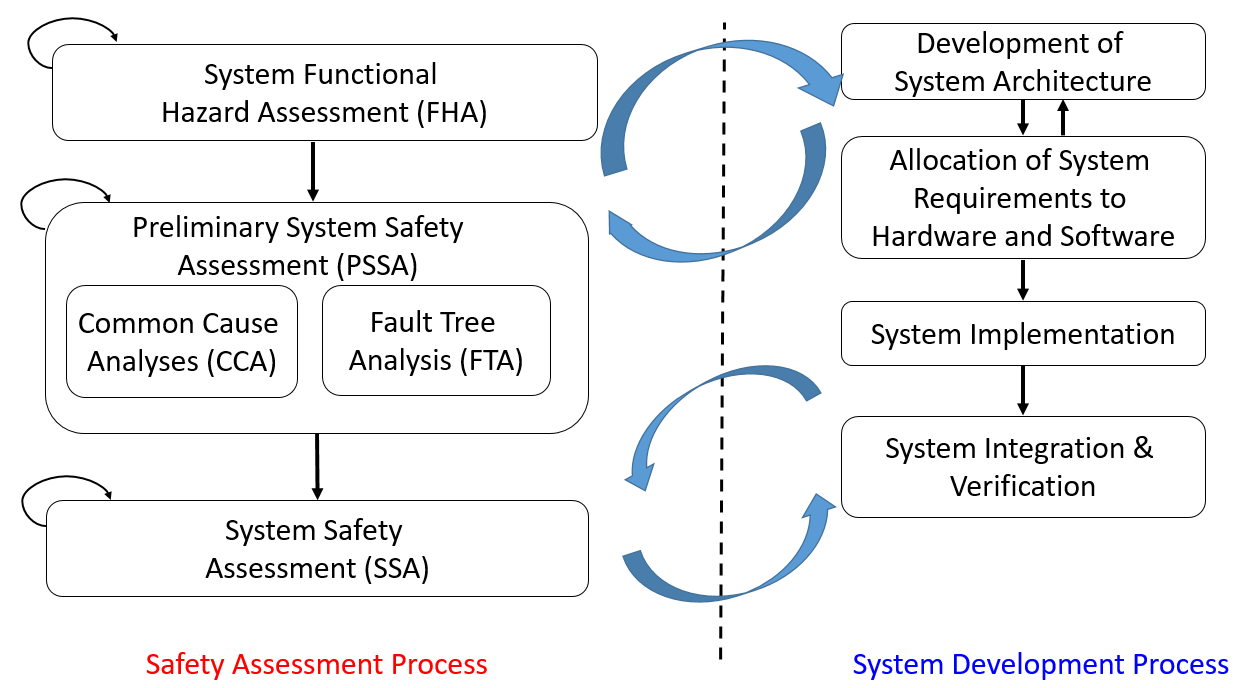
\includegraphics[trim=0 5 0 5,clip,width=0.85\textwidth]{images/process1.png}
	
	\caption{The ARP4754A Safety Assessment Process}
	\label{fig:safety_process}
\end{figure}

\begin{figure}[t!]
	
	\centering
	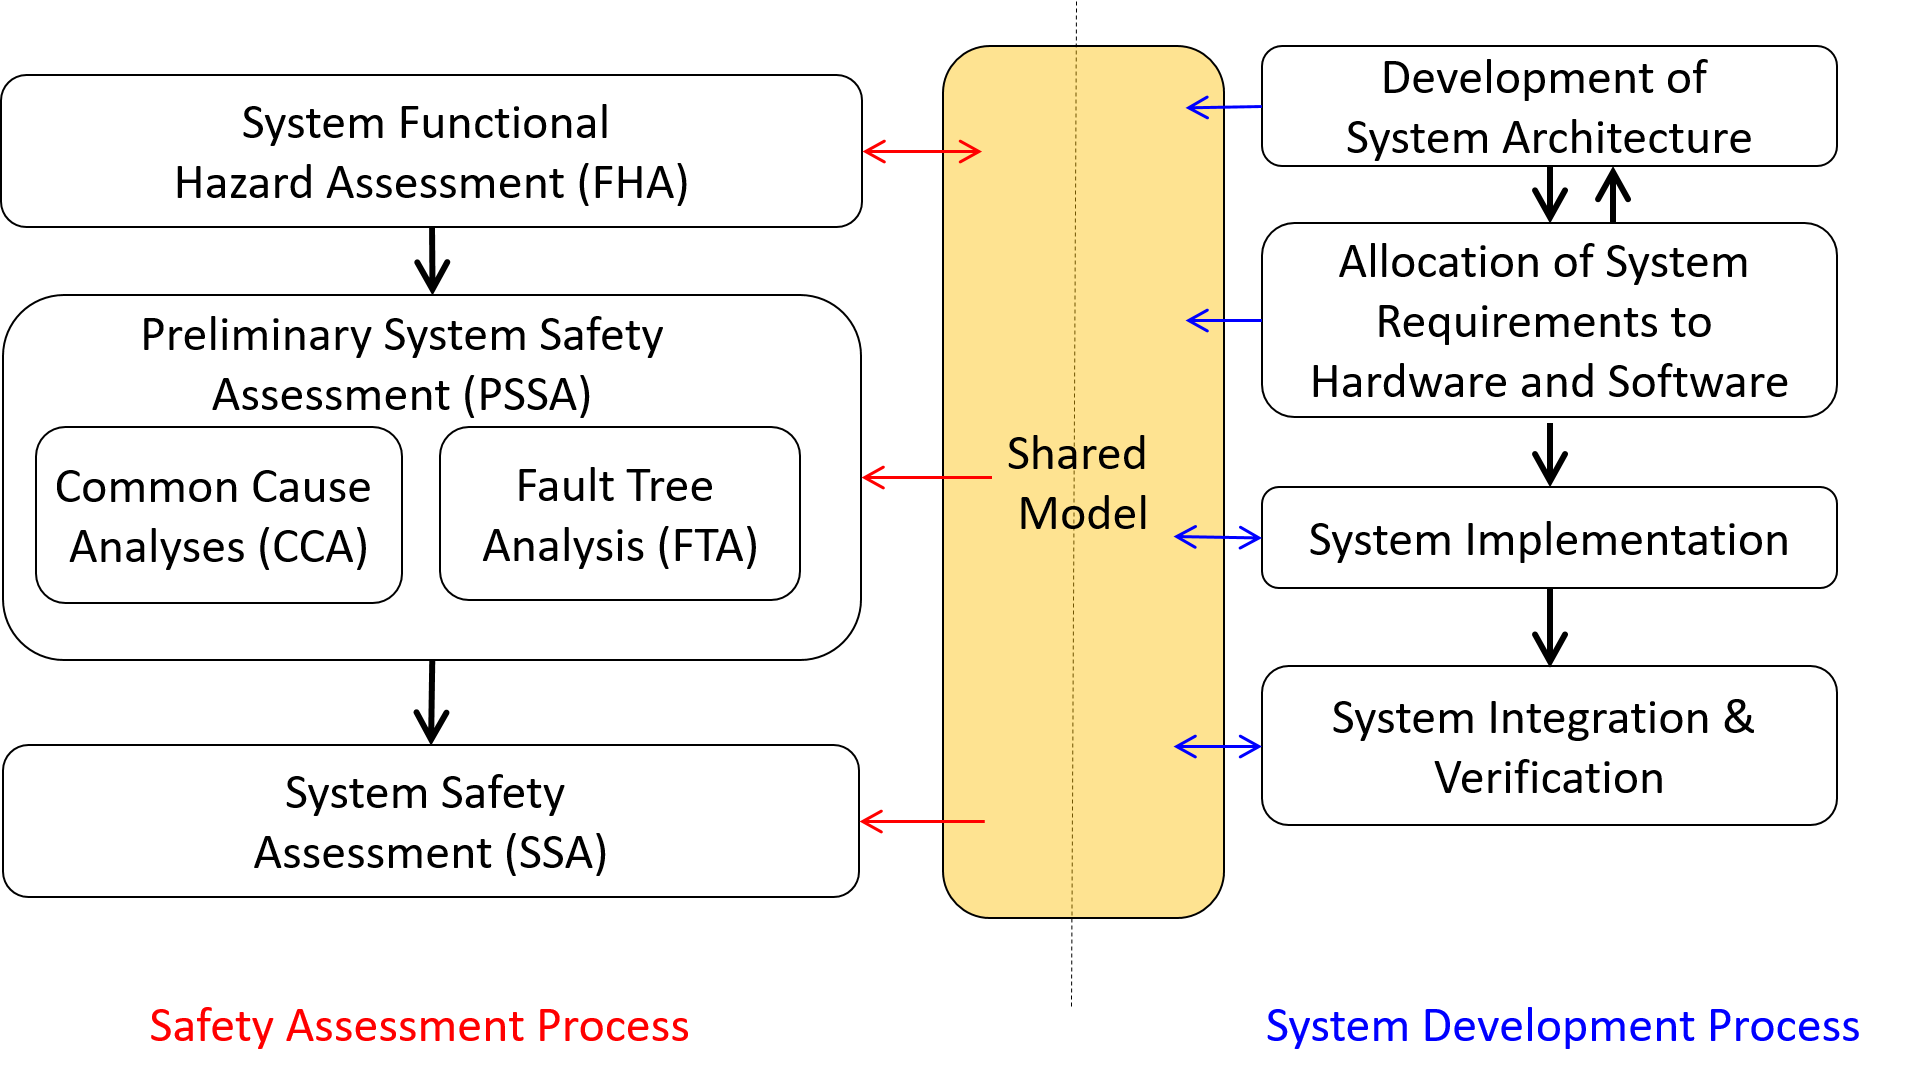
\includegraphics[trim=0 5 0 5,clip,width=0.85\textwidth]{images/process2.png}
	
	\caption{Use of the Shared System/Safety Model in the ARP4754A Safety Assessment Process}
	\label{fig:proposed_safety_process}
\end{figure}
\end{comment}






































\begin{comment}
ARP4761, the Guidelines and Methods for Conducting Safety Assessment Process on Civil Airborne Systems and Equipment, provides guidance on applying development assurance at each hierarchical level throughout the development life cycle of highly-integrated/complex aircraft systems, and has been recognized by the Federal Aviation Administration (FAA) as an acceptable method to establish the assurance process~\cite{SAE:ARP4761}.

\begin{figure*}[h!]
	%\vspace{-0.956in}
	\centering
	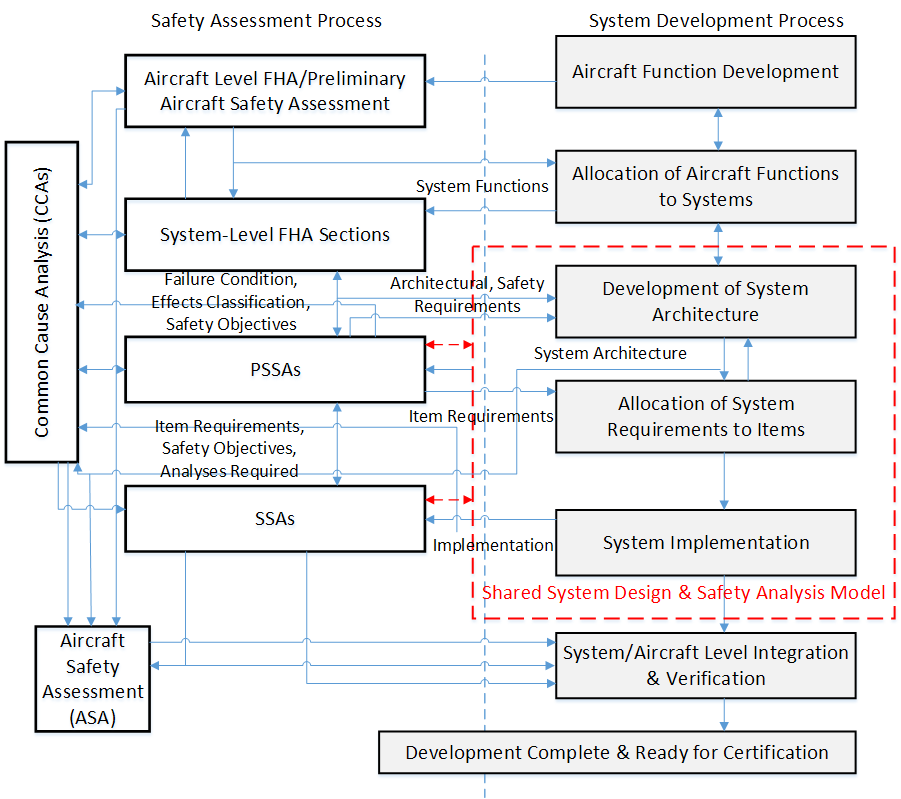
\includegraphics[width=0.7\textwidth]{images/Safety_Assessment_Process.png}
	%\vspace{-0.4in}
	\caption{Using the Shared System/Safety Model in the ARP4754A Safety Assessment Process}
	\label{fig:proposed_safety_process}
\end{figure*}

The safety assessment process is part of the development life cycle, and is tightly coupled with the system development and verification processes. It is used to show compliance with certification requirements and for meeting a company's internal safety standards. The guidelines presented in ARP4761 include various industry accepted safety assessment practices. They are summarized here for convenience. 

\begin{itemize}
\item Functional Hazard Assessment (FHA): This process examines aircraft and system functions to identify potential functional failures and classifies the hazards associated with specific failure conditions. This is usually developed early in the development process and is updated throughout. 

\item Preliminary System Safety Assessment (PSSA): This will establish the system safety requirements and provide some indication that the system architecture can meet those safety requirements. This is also updated throughout the development process.

\item System Safety Assessment (SSA): This process collects, analyzes, and documents verification that the system, as implemented, meets the safety requirements established by the PSSA. 

\item Common Cause Analysis (CCA): The CCA establishes physical and functional separation, isolation, and independence requirements between systems and verifies that these requirements have been met.
\end{itemize}

As shown in Figure~\ref{fig:proposed_safety_process}, these processes occur during the development process and are continually updated throughout. The safety engineers then use the acquired understanding to conduct safety analysis, construct the safety analysis artifacts, and compare the analysis results with established safety objectives and safety-related requirements. 

In practice, prior to performing the safety assessment of a system, the safety engineers are often equipped with the domain knowledge about the system, but do not necessarily have detailed knowledge of how the software functions are designed. Acquiring the required knowledge about the behavior and implementation of each software function in a system can be time-consuming. Industry practitioners have come to realize the benefits and importance of using models to assist the safety assessment process (either by augmenting the existing system design model, or by building a separate safety model), and a revision of the ARP4761 to include model based safety analysis is under way. Capturing failure modes in models and generating safety analysis artifacts directly from models could greatly improve communication and synchronization between system designer and safety engineers, and provide the ability to more accurately analyze complex systems. 

A single unified model to conduct both system development and safety analysis can help reduce the gap in comprehending the system behavior and transferring the knowledge between the system designers and the safety analysts. This maintains a living model that captures the current state of the system design as it moves through the system development lifecycle.

A single unified model also allows all participants of the ARP- \\4754 process to be able to communicate and review the system design using a ``single source of truth.''

A model that supports both system design and safety analysis must describe both the system design information (e.g., system architecture, functional behavior) and safety-relevant information (e.g., failure modes, failure rates).  It must do this in a way that keeps the two types of information distinguishable, yet allows them to interact with each other.

Figure~\ref{fig:proposed_safety_process} presents our proposed use of this shared system design and safety analysis model in the context of the ARP4754A Safety Assessment Process Model (derived from Figure 7 of ARP4754A). The shared model is one of the system development artifacts from the ``Development of System Architecture'' and ``Allocation of System Requirements to Item'' activities in the System Development Process, which interacts with the PSSAs and SSAs activities in the Safety Assessment Process. This is seen as a box labeled ``Shared System Design and Safety model'' on the right column of the figure. The shared model can serve as an interface to capture the information from the system design and implementation that is relevant for the safety analysis.
\end{comment}